% -*- coding:utf-8 -*-
\documentclass[aspectratio=169,10pt]{beamer}
\nonstopmode

% ------------------------------------------------
% Packages
% ------------------------------------------------
\usepackage{xcolor}
\usepackage{xspace}
\usepackage{appendixnumberbeamer}
\usepackage{graphicx}
\usepackage{url}
\usepackage{booktabs}
\usepackage{array}
\usepackage{tikz}
\usetikzlibrary{positioning}
\usepackage{amsmath}

% ------------------------------------------------
% Theme
% ------------------------------------------------
\usetheme[progressbar=frametitle,noslidenumbers]{metropolis}

% ------------------------------------------------
% Color palette
% ------------------------------------------------
\definecolor{navy}{HTML}{182A3A}
\definecolor{teal}{HTML}{2C7A7B}
\definecolor{topgreen}{HTML}{0EAD69}
\definecolor{darkgreen}{HTML}{007A4D}
\definecolor{gold}{HTML}{B8872D}
\definecolor{blue}{HTML}{2F80ED}
\definecolor{gray}{HTML}{5B6670}
\definecolor{light}{HTML}{F5F7FA}
\definecolor{red}{HTML}{A94442}

% ------------------------------------------------
% Beamer colors
% ------------------------------------------------
\setbeamercolor{background canvas}{bg=light}
\setbeamercolor{frametitle}{fg=navy}
\setbeamercolor{title}{fg=navy}
\setbeamercolor{subtitle}{fg=gray}
\setbeamercolor{author}{fg=navy}
\setbeamercolor{institute}{fg=gray}
\setbeamercolor{date}{fg=gray}

\setbeamertemplate{navigation symbols}{}
\setbeamertemplate{footline}{}

% Slide padding
\setbeamersize{text margin left=0.70cm,text margin right=0.70cm}

% ------------------------------------------------
% Graphic paths
% ------------------------------------------------
\graphicspath{{../../plots/}{../../Report Template/template/figures/}{images/}}

% ------------------------------------------------
% Title information
% ------------------------------------------------
\title{Inference of Protein Secondary Structure\\with HMMs and BayesFlow}
\subtitle{Simulation-Based Inference — Project Report}
\author{Armin Maddah Asl \and Samaneh Naghdbishi \and Kiana Ebrahimi Farbod \and Geri Lila}
\institute{TU Dortmund University\\[4pt] \textcolor{gray}{\footnotesize Course Instructor: Prof.\ Dr.\ Paul Bürkner}}
\date{\today}


\begin{document}

% ================================================
% SLIDE 1 — Title page
% ================================================
\begin{frame}[plain]

\begin{tikzpicture}[remember picture,overlay]
  \node[anchor=north west] at ([xshift=0.70cm,yshift=-0.40cm]current page.north west) {
    
\includegraphics[height=8mm]{logo.png}
  };
\end{tikzpicture}

\titlepage
\end{frame}


% ================================================
% SLIDE 2 — Introduction & Modeling Idea
% ================================================
\begin{frame}[plain]

\begin{tikzpicture}[remember picture,overlay]
  \fill[topgreen] (current page.north west) rectangle
    ([yshift=-0.13cm]current page.north east);
  \fill[navy] ([yshift=0.18cm]current page.south west) rectangle
    (current page.south east);
\end{tikzpicture}

\vspace{0.28cm}
\hspace{0.30cm}
\begin{minipage}{0.90\textwidth}

{\large\textbf{\textcolor{navy}{Introduction \& Modeling Idea}}}

\vspace{0.12cm}

\begin{columns}[T,totalwidth=\textwidth]

% ----- LEFT COLUMN -----
\begin{column}{0.50\textwidth}

{\fontsize{9.0}{10.0}\selectfont
\textbf{\textcolor{darkgreen}{The Problem}}
}

\vspace{0.08cm}

{\fontsize{7.5}{9.0}\selectfont
\textcolor{navy}{
Predict per-position secondary structure\\[-0.5mm]
from variable-length amino acid sequences.
}}

\vspace{0.20cm}

{\fontsize{9.0}{10.0}\selectfont
\textbf{\textcolor{darkgreen}{Two-State HMM}}
}

\vspace{0.08cm}

{\fontsize{7.5}{9.0}\selectfont
\textcolor{darkgreen}{State 0} \textcolor{navy}{= $\alpha$-helix}\\[2pt]
\textcolor{gold}{State 1} \textcolor{navy}{= other ($\beta$-sheets \& coils)}
}

\vspace{0.20cm}

{\fontsize{9.0}{10.0}\selectfont
\textbf{\textcolor{darkgreen}{Modeling Goal}}
}

\vspace{0.08cm}

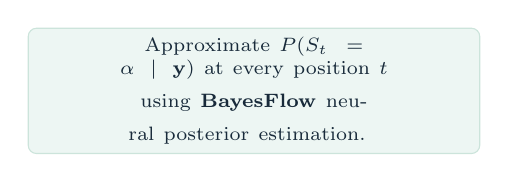
\begin{tikzpicture}
\node[fill=darkgreen!7, draw=darkgreen!20, rounded corners=3pt,
      line width=0.4pt, text width=5.5cm, minimum height=1.0cm, align=center]{
{\fontsize{6.8}{8.0}\selectfont
\textcolor{navy}{
Approximate $P(S_t = \alpha \mid \mathbf{y})$ at every position $t$\\
using \textbf{BayesFlow} neural posterior estimation.
}}
};
\end{tikzpicture}

\end{column}

% ----- RIGHT COLUMN -----
\begin{column}{0.47\textwidth}

{\fontsize{9.0}{10.0}\selectfont
\textbf{\textcolor{darkgreen}{Overall Pipeline}}
}

\vspace{0.12cm}

% Pipeline as vertical blocks
\begin{center}
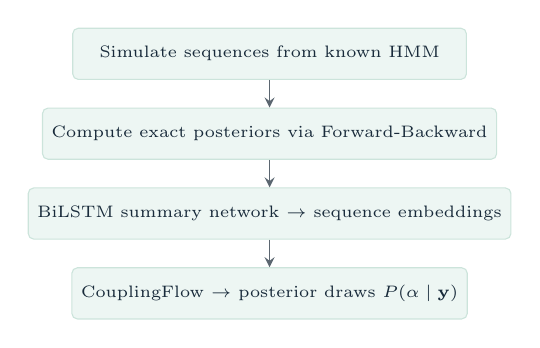
\begin{tikzpicture}[
  box/.style={fill=darkgreen!7, draw=darkgreen!20, rounded corners=2pt,
              line width=0.4pt, minimum width=5.0cm, minimum height=0.65cm,
              font=\fontsize{6.5}{7.5}\selectfont, align=center, text=navy},
  arrow/.style={->, >=stealth, line width=0.6pt, color=gray}
]

\node[box] (s1) {Simulate sequences from known HMM};
\node[box, below=0.35cm of s1] (s2) {Compute exact posteriors via Forward-Backward};
\node[box, below=0.35cm of s2] (s3) {BiLSTM summary network $\to$ sequence embeddings};
\node[box, below=0.35cm of s3] (s4) {CouplingFlow $\to$ posterior draws $P(\alpha \mid \mathbf{y})$};

\draw[arrow] (s1) -- (s2);
\draw[arrow] (s2) -- (s3);
\draw[arrow] (s3) -- (s4);

\end{tikzpicture}
\end{center}

\vspace{0.15cm}

{\fontsize{9.0}{10.0}\selectfont
\textbf{\textcolor{darkgreen}{Validation}}
}

\vspace{0.08cm}

{\fontsize{7.2}{8.5}\selectfont
\textcolor{navy}{
Compare to experimental ground truth:\\[-0.5mm]
Human insulin \textbf{1A7F} (chain A: 21 aa, chain B: 29 aa).
}}

\end{column}

\end{columns}

\end{minipage}

\vfill
\hspace{0.95cm}
{\fontsize{5.5}{6.0}\selectfont\textcolor{gray}{SBI Project | 2/12}}
\vspace{0.26cm}

\end{frame}


% ================================================
% SLIDE 3 — The 2-State Hidden Markov Model
% ================================================
\begin{frame}[plain]

\begin{tikzpicture}[remember picture,overlay]
  \fill[topgreen] (current page.north west) rectangle
    ([yshift=-0.13cm]current page.north east);
  \fill[navy] ([yshift=0.18cm]current page.south west) rectangle
    (current page.south east);
\end{tikzpicture}

\vspace{0.28cm}
\hspace{0.30cm}
\begin{minipage}{0.90\textwidth}

{\large\textbf{\textcolor{navy}{The 2-State Hidden Markov Model}}}

\vspace{0.06cm}

\begin{columns}[T,totalwidth=\textwidth]

% ==================== LEFT COLUMN: State Transitions (visual anchor) ====================
\begin{column}{0.50\textwidth}

{\fontsize{7.5}{8.5}\selectfont
\textbf{\textcolor{darkgreen}{State Transitions}}
}

\vspace{0.14cm}

% Enlarged transition diagram — the hero of this slide
\begin{center}
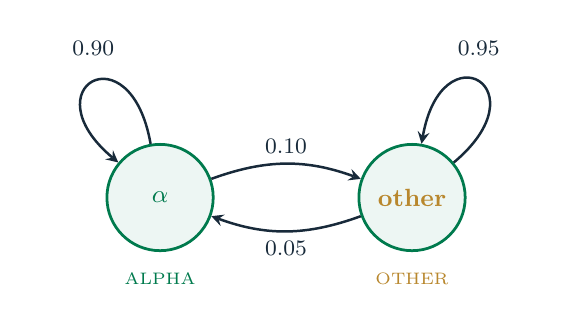
\begin{tikzpicture}[
  state/.style={circle, draw=darkgreen, fill=darkgreen!7, line width=1.0pt,
                minimum size=1.35cm, font=\fontsize{9}{11}\selectfont\bfseries},
  arrow/.style={->, >=stealth, line width=0.9pt, color=navy},
  label/.style={font=\fontsize{8}{10}\selectfont, text=navy}
]

\node[state, text=darkgreen] (a) at (0,0) {$\alpha$};
\node[state, text=gold] (o) at (3.2,0) {other};

\draw[arrow] (a) edge[loop, out=100, in=140, looseness=8] node[label, above=0.20cm] {0.90} (a);
\draw[arrow] (o) edge[loop, out=40, in=80, looseness=8] node[label, above=0.20cm] {0.95} (o);
\draw[arrow] (a) to[bend left=20] node[label, above] {0.10} (o);
\draw[arrow] (o) to[bend left=20] node[label, below] {0.05} (a);

\node[below=0.14cm of a, font=\fontsize{6.5}{7.5}\selectfont, text=darkgreen] {ALPHA};
\node[below=0.14cm of o, font=\fontsize{6.5}{7.5}\selectfont, text=gold] {OTHER};
\end{tikzpicture}
\end{center}

\vspace{0.16cm}

{\fontsize{6.5}{7.5}\selectfont
\textcolor{navy}{
\textbf{Deterministic start:} $P(S_1=\text{other})=1.0,\ P(S_1=\alpha)=0.0$\\[3pt]
\textbf{Highly persistent:} $\alpha$ stays $\alpha$ (90\%), other stays other (95\%)
}}

\end{column}

% ==================== RIGHT COLUMN: Emissions + Prior ====================
\begin{column}{0.46\textwidth}

% --- Selected Emission Contrasts ---
{\fontsize{7.5}{8.5}\selectfont
\textbf{\textcolor{darkgreen}{Selected Emission Contrasts}}
}

\vspace{0.06cm}

{\fontsize{6.5}{7.5}\selectfont
\begin{tabular}{lccc}
\toprule
Amino acid & $\alpha$-helix & other & Role \\
\midrule
\textbf{A} (Alanine)  & \textcolor{darkgreen}{12\%} & 6\%  & Strong former \\
\textbf{E} (Glutamic) & \textcolor{darkgreen}{9\%}  & 5\%  & Former \\
\textbf{P} (Proline)  & 2\%  & \textcolor{red}{6\%}  & Breaker \\
\textbf{G} (Glycine)  & 4\%  & \textcolor{red}{9\%}  & Breaker \\
\bottomrule
\end{tabular}
}

\vspace{0.04cm}

{\fontsize{5.5}{6.5}\selectfont
\textcolor{gray}{Full $20 \times 2$ table in written report.}
}

% --- Prior Dynamics ---
\vspace{0.16cm}

{\fontsize{7.5}{8.5}\selectfont
\textbf{\textcolor{darkgreen}{Prior Dynamics}}
}

\vspace{0.06cm}

{\fontsize{6.8}{8.0}\selectfont
\textcolor{navy}{
\textbf{Stationary distribution:}\\[2pt]
$\pi(\alpha)=0.05/(0.05+0.10)=1/3\approx 33\%$\\[2pt]
$\pi(\text{other})\approx 67\%$
}}

\vspace{0.06cm}


\begin{tikzpicture}
\node[fill=darkgreen!7, draw=darkgreen!20, rounded corners=3pt,
      line width=0.4pt, text width=5.2cm, minimum height=0.55cm, align=center]{
{\fontsize{6.2}{7.2}\selectfont
\textcolor{navy}{
Prior strongly favors \textbf{non-helical} states ($\sim$67\%).
}}
};
\end{tikzpicture}

\end{column}

\end{columns}

\end{minipage}

\vfill
\hspace{0.95cm}
{\fontsize{5.5}{6.0}\selectfont\textcolor{gray}{SBI Project | 3/12}}
\vspace{0.26cm}

\note{%
\textbf{Slide 3 --- the two-state HMM.}
Hidden states are $\alpha$-helix and ``other'' (sheets + coils); the transition matrix is
fixed and known --- set by hand, never fitted.
Both states are highly self-persistent (0.90 and 0.95 on the diagonal), so the chain
emits contiguous runs, like real secondary-structure segments.
Derive the stationary distribution from $\pi P = \pi$: with exit rates $0.10$
($\alpha\!\to$other) and $0.05$ (other$\to\alpha$), balance gives
$\pi(\alpha) = 0.05/(0.05+0.10) = 1/3 \approx 33\%$, so $\pi(\text{other}) \approx 67\%$
--- the prior favours non-helix roughly 2:1.
Emissions differ by state: alanine and glutamate are formers (higher $\alpha$
probability), proline and glycine are breakers (higher under ``other''); the full
$20\times2$ table is in the written report.
}

\end{frame}


% ================================================
% SLIDE 4 — Data Generation & Analytical Targets
% ================================================
\begin{frame}[plain]

\begin{tikzpicture}[remember picture,overlay]
  \fill[topgreen] (current page.north west) rectangle
    ([yshift=-0.13cm]current page.north east);
  \fill[navy] ([yshift=0.18cm]current page.south west) rectangle
    (current page.south east);
\end{tikzpicture}

\vspace{0.28cm}
\hspace{0.30cm}
\begin{minipage}{0.90\textwidth}

{\large\textbf{\textcolor{navy}{Data Generation \& Analytical Targets}}}

\vspace{0.12cm}

\begin{columns}[T,totalwidth=\textwidth]

% ----- LEFT -----
\begin{column}{0.48\textwidth}

{\fontsize{8.5}{10.0}\selectfont
\textbf{\textcolor{darkgreen}{Simulator}}
}

\vspace{0.06cm}

{\fontsize{7.0}{8.5}\selectfont
\textcolor{navy}{
Sequential Markov sampling of hidden states.\\[2pt]
Independent randomized emission draws.\\[2pt]
Random sequence lengths: 10–60 aa.\\[2pt]
\textbf{100\% simulated} — no real proteins.
}}

\vspace{0.18cm}

{\fontsize{8.5}{10.0}\selectfont
\textbf{\textcolor{darkgreen}{Target Computation}}
}

\vspace{0.06cm}

{\fontsize{7.0}{8.5}\selectfont
\textcolor{navy}{
Exact posteriors via Forward-Backward.\\[2pt]
\texttt{hmmlearn.CategoricalHMM} — manually\\[1pt]
configured, never \texttt{.fit()}.
}}

\vspace{0.18cm}

{\fontsize{8.5}{10.0}\selectfont
\textbf{\textcolor{darkgreen}{Verification}}
}

\vspace{0.06cm}

{\fontsize{7.0}{8.5}\selectfont
\textcolor{navy}{
Targets verified against independent\\[2pt]
pure-NumPy FB solver. Confirms:\\[2pt]
$P(S_0 = \alpha) \equiv 0$ (position 0 = seq.\ position 1).
}}

\end{column}

% ----- RIGHT -----
\begin{column}{0.48\textwidth}

{\fontsize{8.5}{10.0}\selectfont
\textbf{\textcolor{darkgreen}{On-demand Generation}}
}

\vspace{0.06cm}

{\fontsize{7.0}{8.5}\selectfont
\textcolor{navy}{
\texttt{generate\_dataset(n, \ldots)} produces\\[2pt]
any number of \texttt{(sequence, posterior,}\\[1pt]
\texttt{states)} tuples. Downstream code\\[2pt]
chooses the split sizes.
}}

\vspace{0.18cm}

{\fontsize{8.5}{10.0}\selectfont
\textbf{\textcolor{darkgreen}{Variable-Length by Design}}
}

\vspace{0.08cm}

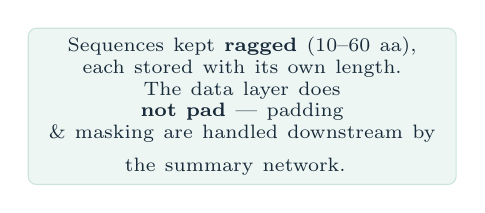
\begin{tikzpicture}
\node[fill=darkgreen!7, draw=darkgreen!20, rounded corners=3pt,
      line width=0.4pt, text width=5.2cm, minimum height=0.85cm, align=center]{
{\fontsize{6.8}{7.8}\selectfont
\textcolor{navy}{
Sequences kept \textbf{ragged} (10–60 aa),\\
each stored with its own length.\\
The data layer does \textbf{not pad} — padding\\
\& masking are handled downstream by\\
the summary network.
}}
};
\end{tikzpicture}

\vspace{0.12cm}

{\fontsize{8.5}{10.0}\selectfont
\textbf{\textcolor{darkgreen}{Storage}}
}

\vspace{0.06cm}

{\fontsize{7.0}{8.5}\selectfont
\textcolor{navy}{
\texttt{.npz} format: concatenated arrays +\\[2pt]
\texttt{lengths} vector. No object arrays.
}}

\end{column}

\end{columns}

\end{minipage}

\vfill
\hspace{0.95cm}
{\fontsize{5.5}{6.0}\selectfont\textcolor{gray}{SBI Project | 4/12}}
\vspace{0.26cm}

\note{%
\textbf{Slide 4 --- data generation.}
The simulator draws hidden states by Markov sampling, then emits amino acids
independently at each position; lengths are uniform on 10--60 aa and everything is
100\% simulated --- no real proteins.
Targets are the exact per-position posteriors $P(S_t = \alpha \mid \mathbf{y})$ from the
Forward--Backward algorithm via \texttt{hmmlearn.CategoricalHMM}, with parameters set by
hand (never \texttt{.fit()}). Emphasise that these targets are \emph{deterministic}: the
same sequence always yields the same posterior --- there is no sampling noise.
Position~0 is forced: because the start distribution puts all mass on ``other'',
$P(S_0 = \alpha) \equiv 0$ --- a clean sanity check, and we verify every target against an
independent pure-NumPy Forward--Backward solver.
Data is stored ragged (each sequence with its own length); padding and masking are
deliberately deferred to Member~2's summary network. \texttt{generate\_dataset(n, \ldots)}
yields any number of tuples --- the 800/200/200 split lives in the downstream training and
diagnostics code, not in this data layer.
}

\end{frame}


% ================================================
% SLIDE 5 — The Summary Network (BiLSTM)
% ================================================
\begin{frame}[plain]

\begin{tikzpicture}[remember picture,overlay]
  \fill[topgreen] (current page.north west) rectangle
    ([yshift=-0.13cm]current page.north east);
  \fill[navy] ([yshift=0.18cm]current page.south west) rectangle
    (current page.south east);
\end{tikzpicture}

\vspace{0.28cm}
\hspace{0.30cm}
\begin{minipage}{0.90\textwidth}

{\large\textbf{\textcolor{navy}{The Summary Network — BiLSTM}}}

\vspace{0.12cm}

% Architecture diagram — larger, the hero of this slide
\begin{center}
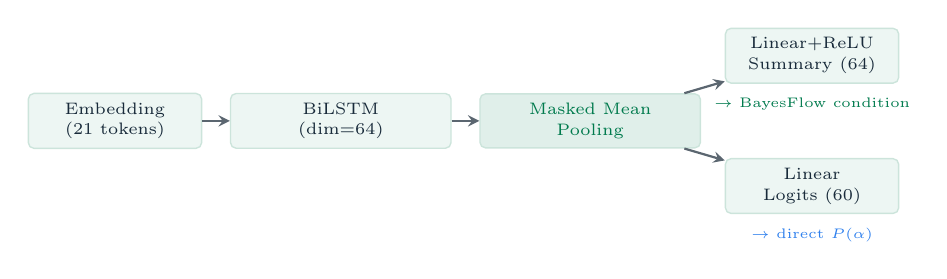
\begin{tikzpicture}[
  box/.style={fill=darkgreen!7, draw=darkgreen!20, rounded corners=2pt,
              line width=0.5pt, minimum height=0.60cm,
              font=\fontsize{6.5}{7.5}\selectfont, align=center, text=navy},
  callout/.style={fill=red!4, draw=red!25, rounded corners=1pt,
                  font=\fontsize{5.8}{6.5}\selectfont, text=navy, align=center},
  arrow/.style={->, >=stealth, line width=0.8pt, color=gray},
  node distance=0.35cm
]

\node[box, minimum width=2.2cm] (emb) {Embedding\\(21 tokens)};
\node[box, minimum width=2.8cm, right=of emb] (lstm) {BiLSTM\\(dim=64)};
\node[box, minimum width=2.8cm, right=of lstm, text=darkgreen, fill=darkgreen!12] (mask) {Masked Mean\\Pooling};
\node[box, minimum width=2.2cm, above right=0.12cm and 0.3cm of mask] (sum) {Linear+ReLU\\Summary (64)};
\node[box, minimum width=2.2cm, below right=0.12cm and 0.3cm of mask] (pos) {Linear\\Logits (60)};

\draw[arrow] (emb) -- (lstm);
\draw[arrow] (lstm) -- (mask);
\draw[arrow] (mask) -- (sum);
\draw[arrow] (mask) -- (pos);

% Labels on the diagram
\node[below=0.05cm of sum, font=\fontsize{5.5}{6}\selectfont, text=darkgreen] {$\to$ BayesFlow condition};
\node[below=0.05cm of pos, font=\fontsize{5.5}{6}\selectfont, text=blue] {$\to$ direct $P(\alpha)$};

\end{tikzpicture}
\end{center}

\vspace{0.14cm}

% 3 clean takeaways — no bullets, just clear statements
\begin{center}
{\fontsize{7.0}{8.5}\selectfont
\textcolor{navy}{
\textbf{1.} BiLSTM captures \textbf{sequential} dependencies — permutation-invariant nets fail here.\\[6pt]
\textbf{2.} Padding token 20 \& masked loss $\to$ handles variable-length sequences.\\[6pt]
\textbf{3.} Two-stage: BiLSTM pretrained on BCE $\to$ frozen $\to$ CouplingFlow on top.
}}
\end{center}

\vspace{0.06cm}


\end{minipage}

\vfill
\hspace{0.95cm}
{\fontsize{5.5}{6.0}\selectfont\textcolor{gray}{SBI Project | 5/12}}
\vspace{0.26cm}

\end{frame}


% ================================================
% SLIDE 6 — Two-Stage Training & CouplingFlow
% ================================================
\begin{frame}[plain]

\begin{tikzpicture}[remember picture,overlay]
  \fill[topgreen] (current page.north west) rectangle
    ([yshift=-0.13cm]current page.north east);
  \fill[navy] ([yshift=0.18cm]current page.south west) rectangle
    (current page.south east);
\end{tikzpicture}

\vspace{0.28cm}
\hspace{0.30cm}
\begin{minipage}{0.90\textwidth}

{\large\textbf{\textcolor{navy}{Two-Stage Training \& CouplingFlow}}}

\vspace{0.22cm}

{\fontsize{7.5}{8.5}\selectfont
\textbf{\textcolor{darkgreen}{Training Pipeline}}
}

\vspace{0.12cm}

\begin{center}
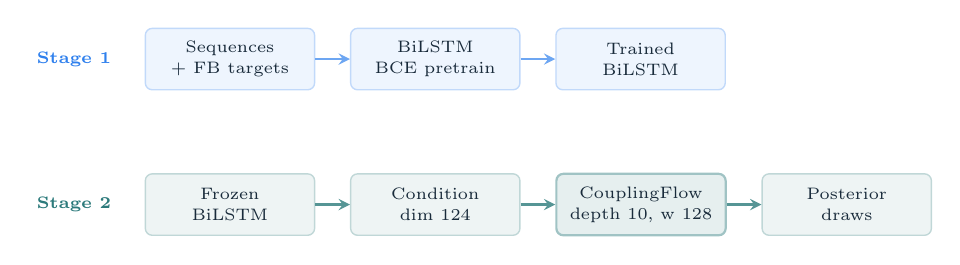
\begin{tikzpicture}[
  box/.style={rounded corners=2.5pt, line width=0.5pt,
              minimum height=0.78cm, minimum width=2.15cm,
              font=\fontsize{6.5}{7.6}\selectfont, align=center, text=navy},
  arrow/.style={->, >=stealth, line width=0.8pt},
  node distance=0.44cm
]

% --- Stage 1 ---
\node[box, fill=blue!8,  draw=blue!30] (s1a) {Sequences\\$+$ FB targets};
\node[box, fill=blue!8,  draw=blue!30, right=of s1a] (s1b) {BiLSTM\\BCE pretrain};
\node[box, fill=blue!8,  draw=blue!30, right=of s1b] (s1c) {Trained\\BiLSTM};
\draw[arrow, color=blue!70] (s1a) -- (s1b);
\draw[arrow, color=blue!70] (s1b) -- (s1c);
\node[left=0.30cm of s1a, font=\fontsize{6.2}{7}\selectfont, text=blue] {\textbf{Stage 1}};

% --- Stage 2 ---
\node[box, fill=teal!8, draw=teal!30, below=1.05cm of s1a] (s2a) {Frozen\\BiLSTM};
\node[box, fill=teal!8, draw=teal!30, right=of s2a] (s2b) {Condition\\dim 124};
\node[box, fill=teal!12, draw=teal!45, line width=0.8pt, right=of s2b] (s2c) {CouplingFlow\\depth 10, w 128};
\node[box, fill=teal!8, draw=teal!30, right=of s2c] (s2d) {Posterior\\draws};
\draw[arrow, color=teal!80] (s2a) -- (s2b);
\draw[arrow, color=teal!80] (s2b) -- (s2c);
\draw[arrow, color=teal!80] (s2c) -- (s2d);
\node[left=0.30cm of s2a, font=\fontsize{6.2}{7}\selectfont, text=teal] {\textbf{Stage 2}};


\end{tikzpicture}
\end{center}

\vspace{0.16cm}

{\fontsize{7.5}{8.5}\selectfont
\textbf{\textcolor{darkgreen}{Key Design Decisions}}
}

\vspace{0.10cm}

\begin{center}
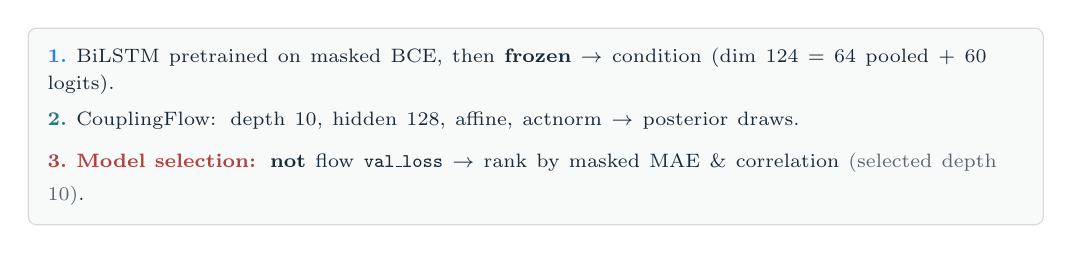
\begin{tikzpicture}
\node[fill=navy!3, draw=navy!18, rounded corners=3pt, line width=0.4pt,
      text width=12.4cm, inner sep=7pt, align=left]{
{\fontsize{7.2}{10.0}\selectfont
\textcolor{navy}{
\textcolor{blue}{\textbf{1.}}~BiLSTM pretrained on masked BCE, then \textbf{frozen} $\to$ condition (dim 124 $=$ 64 pooled $+$ 60 logits).\\[3pt]
\textcolor{teal}{\textbf{2.}}~CouplingFlow: depth~10, hidden~128, affine, actnorm $\to$ posterior draws.\\[3pt]
\textcolor{red}{\textbf{3.}}~\textcolor{red}{\textbf{Model selection:}} \textbf{not} flow \texttt{val\_loss} $\to$ rank by masked MAE \& correlation \textcolor{gray}{(selected depth 10)}.
}}
};
\end{tikzpicture}
\end{center}

\end{minipage}

\vfill
\hspace{0.95cm}
{\fontsize{5.5}{6.0}\selectfont\textcolor{gray}{SBI Project | 6/12}}

\end{frame}

% ================================================
% SLIDE 7 — Diagnostics: Adapted SBC
% ================================================
\begin{frame}[plain]

\begin{tikzpicture}[remember picture,overlay]
  \fill[topgreen] (current page.north west) rectangle
    ([yshift=-0.13cm]current page.north east);
  \fill[navy] ([yshift=0.18cm]current page.south west) rectangle
    (current page.south east);
\end{tikzpicture}

\vspace{0.28cm}
\hspace{0.30cm}
\begin{minipage}{0.90\textwidth}

{\large\textbf{\textcolor{navy}{Diagnostics: Adapted Simulation-Based Calibration}}}

\vspace{0.10cm}

\begin{columns}[T,totalwidth=\textwidth]

% ----- LEFT: Challenge -----
\begin{column}{0.45\textwidth}

{\fontsize{8.5}{10.0}\selectfont
\textbf{\textcolor{darkgreen}{Standard SBC}}
}

\vspace{0.06cm}

{\fontsize{7.0}{8.2}\selectfont
\textcolor{navy}{
Draw $\boldsymbol{\theta} \sim p(\boldsymbol{\theta})$ from prior.\\[2pt]
Simulate data $\mathbf{x} \sim p(\mathbf{x} \mid \boldsymbol{\theta})$.\\[2pt]
Compute posterior, check if ranks of\\[-0.5mm]
$\boldsymbol{\theta}_{\text{true}}$ are uniform.
}}

\vspace{0.18cm}

{\fontsize{8.5}{10.0}\selectfont
\textbf{\textcolor{red}{Our Challenge}}
}

\vspace{0.06cm}

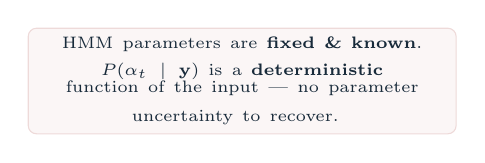
\begin{tikzpicture}
\node[fill=red!5, draw=red!20, rounded corners=3pt,
      line width=0.4pt, text width=5.2cm, minimum height=1.3cm, align=center]{
{\fontsize{6.5}{7.5}\selectfont
\textcolor{navy}{
HMM parameters are \textbf{fixed \& known}.\\[2pt]
$P(\alpha_t \mid \mathbf{y})$ is a \textbf{deterministic}\\[-0.5mm]
function of the input — no parameter\\[-0.5mm]
uncertainty to recover.
}}
};
\end{tikzpicture}

\end{column}

% ----- RIGHT: Our Method -----
\begin{column}{0.52\textwidth}

{\fontsize{8.5}{10.0}\selectfont
\textbf{\textcolor{darkgreen}{Our Adapted Method}}
}

\vspace{0.08cm}

% Steps as numbered boxes
\begin{center}
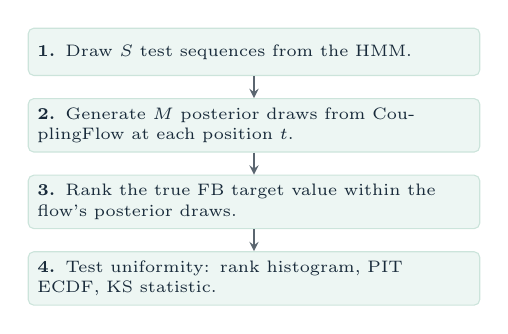
\begin{tikzpicture}[
  sbox/.style={fill=darkgreen!7, draw=darkgreen!20, rounded corners=2pt,
               line width=0.4pt, text width=5.5cm, minimum height=0.60cm,
               font=\fontsize{6.3}{7.3}\selectfont, align=left, text=navy},
  arrow/.style={->, >=stealth, line width=0.5pt, color=gray}
]

\node[sbox] (s1) {\textbf{1.} Draw $S$ test sequences from the HMM.};
\node[sbox, below=0.28cm of s1] (s2) {\textbf{2.} Generate $M$ posterior draws from CouplingFlow at each position $t$.};
\node[sbox, below=0.28cm of s2] (s3) {\textbf{3.} Rank the true FB target value within the flow's posterior draws.};
\node[sbox, below=0.28cm of s3] (s4) {\textbf{4.} Test uniformity: rank histogram, PIT ECDF, KS statistic.};

\draw[arrow] (s1) -- (s2);
\draw[arrow] (s2) -- (s3);
\draw[arrow] (s3) -- (s4);

\end{tikzpicture}
\end{center}

\vspace{0.12cm}

{\fontsize{8.5}{10.0}\selectfont
\textbf{\textcolor{darkgreen}{What This Tests}}
}

\vspace{0.06cm}

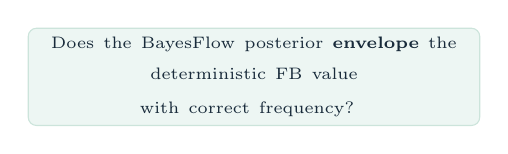
\begin{tikzpicture}
\node[fill=darkgreen!7, draw=darkgreen!20, rounded corners=3pt,
      line width=0.4pt, text width=5.5cm, minimum height=0.70cm, align=center]{
{\fontsize{6.5}{7.5}\selectfont
\textcolor{navy}{
Does the BayesFlow posterior \textbf{envelope} the\\[-0.3mm]
deterministic FB value with correct frequency?
}}
};
\end{tikzpicture}

\vspace{0.12cm}

{\fontsize{6.5}{7.5}\selectfont
\textcolor{gray}{
Note: Not a classical prior-predictive SBC — adapted for the deterministic-target setting.
}}

\end{column}

\end{columns}

\end{minipage}

\vfill
\hspace{0.95cm}
{\fontsize{5.5}{6.0}\selectfont\textcolor{gray}{SBI Project | 7/12}}
\vspace{0.26cm}

\end{frame}


% ================================================
% SLIDE 8 — Calibration Results: Adapted SBC
% ================================================
\begin{frame}[plain]

\begin{tikzpicture}[remember picture,overlay]
  \fill[topgreen] (current page.north west) rectangle
    ([yshift=-0.13cm]current page.north east);
  \fill[navy] ([yshift=0.18cm]current page.south west) rectangle
    (current page.south east);
\end{tikzpicture}

\vspace{0.28cm}
\hspace{0.30cm}
\begin{minipage}{0.90\textwidth}

{\large\textbf{\textcolor{navy}{Calibration Results — Adapted SBC}}}

\vspace{0.12cm}

\begin{columns}[T,totalwidth=\textwidth]

% ----- LEFT: Big Plot (70%) -----
\begin{column}{0.68\textwidth}

\begin{center}
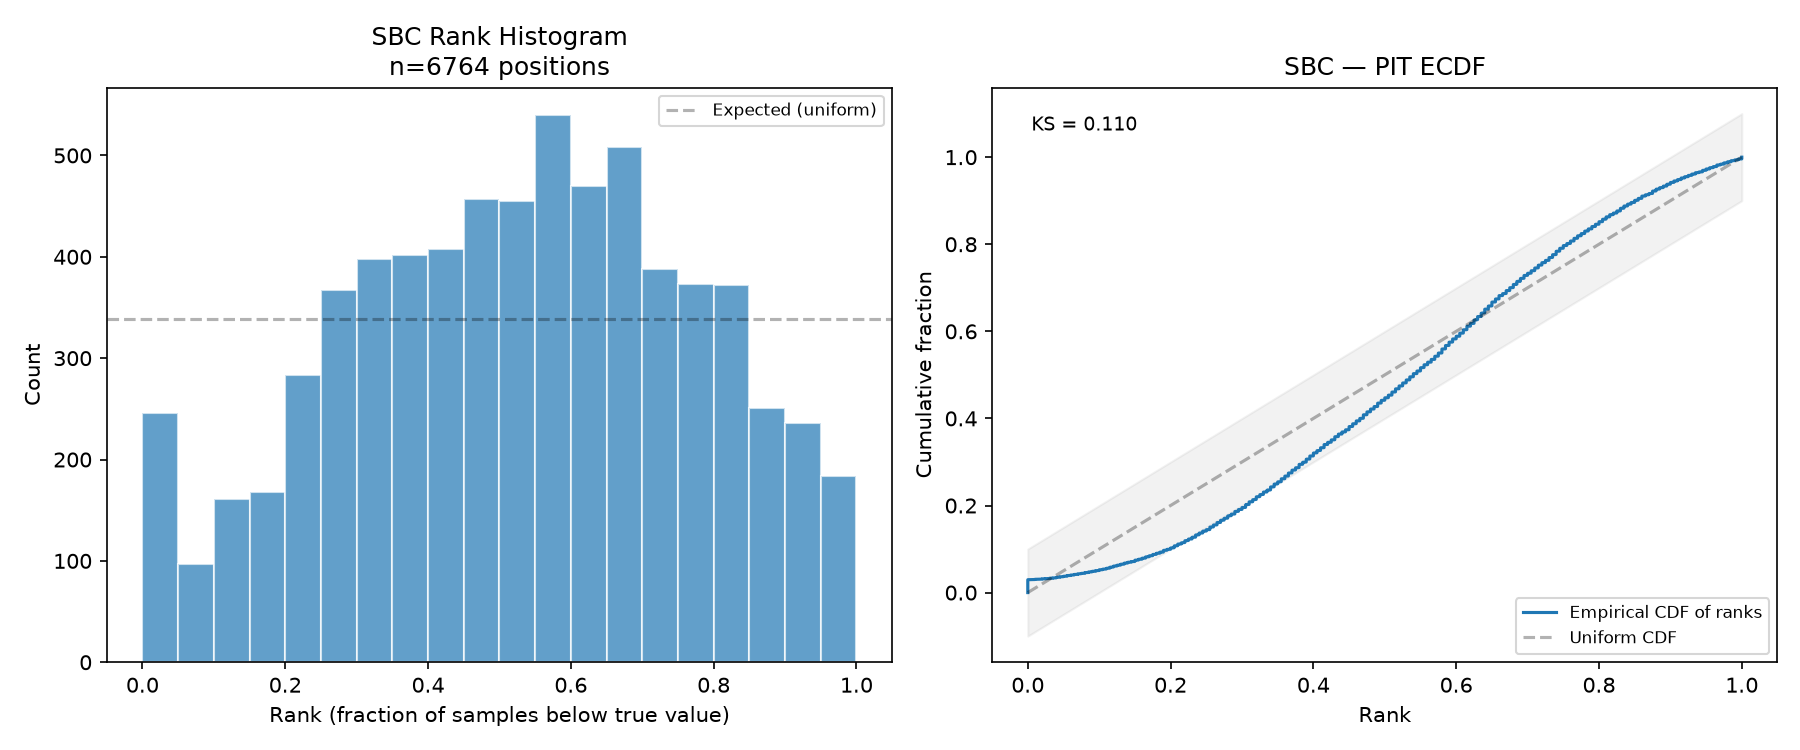
\includegraphics[width=\linewidth,height=0.62\textheight,keepaspectratio]{sbc.png}
\end{center}

\end{column}

% ----- RIGHT: Headline (30%) -----
\begin{column}{0.29\textwidth}

{\fontsize{9.0}{10.5}\selectfont
\textbf{\textcolor{red}{Systematic Underestimation}}
}

\vspace{0.12cm}

{\fontsize{7.5}{9.0}\selectfont
\textcolor{navy}{
Rank histogram shifted \textbf{rightward}:\\[3pt]
mean rank = \textbf{0.65}\\[1pt]
only \textbf{27\%} below 0.50\\[6pt]
\textcolor{red}{KS = \textbf{0.234}}
}}

\vspace{0.25cm}

{\fontsize{7.5}{9.0}\selectfont
\textcolor{navy}{
True FB $P(\alpha)$ is frequently\\[-0.3mm]
\textbf{larger} than posterior draws.\\[3pt]
$\to$ Padded zero boundaries pull\\[-0.3mm]
the continuous flow toward 0.
}}

\end{column}

\end{columns}

\end{minipage}

\vfill
\hspace{0.95cm}
{\fontsize{5.5}{6.0}\selectfont\textcolor{gray}{SBI Project | 8/12}}
\vspace{0.26cm}

\end{frame}


% ================================================
% SLIDE 9 — Calibration Results: Z-Score & Coverage
% ================================================
\begin{frame}[plain]

\begin{tikzpicture}[remember picture,overlay]
  \fill[topgreen] (current page.north west) rectangle
    ([yshift=-0.13cm]current page.north east);
  \fill[navy] ([yshift=0.18cm]current page.south west) rectangle
    (current page.south east);
\end{tikzpicture}

\vspace{0.28cm}
\hspace{0.30cm}
\begin{minipage}{0.90\textwidth}

{\large\textbf{\textcolor{navy}{Calibration Results — Z-Score \& Coverage}}}

\vspace{0.12cm}

\begin{columns}[T,totalwidth=\textwidth]

% ----- LEFT: Big Plot (70%) -----
\begin{column}{0.68\textwidth}

\begin{center}
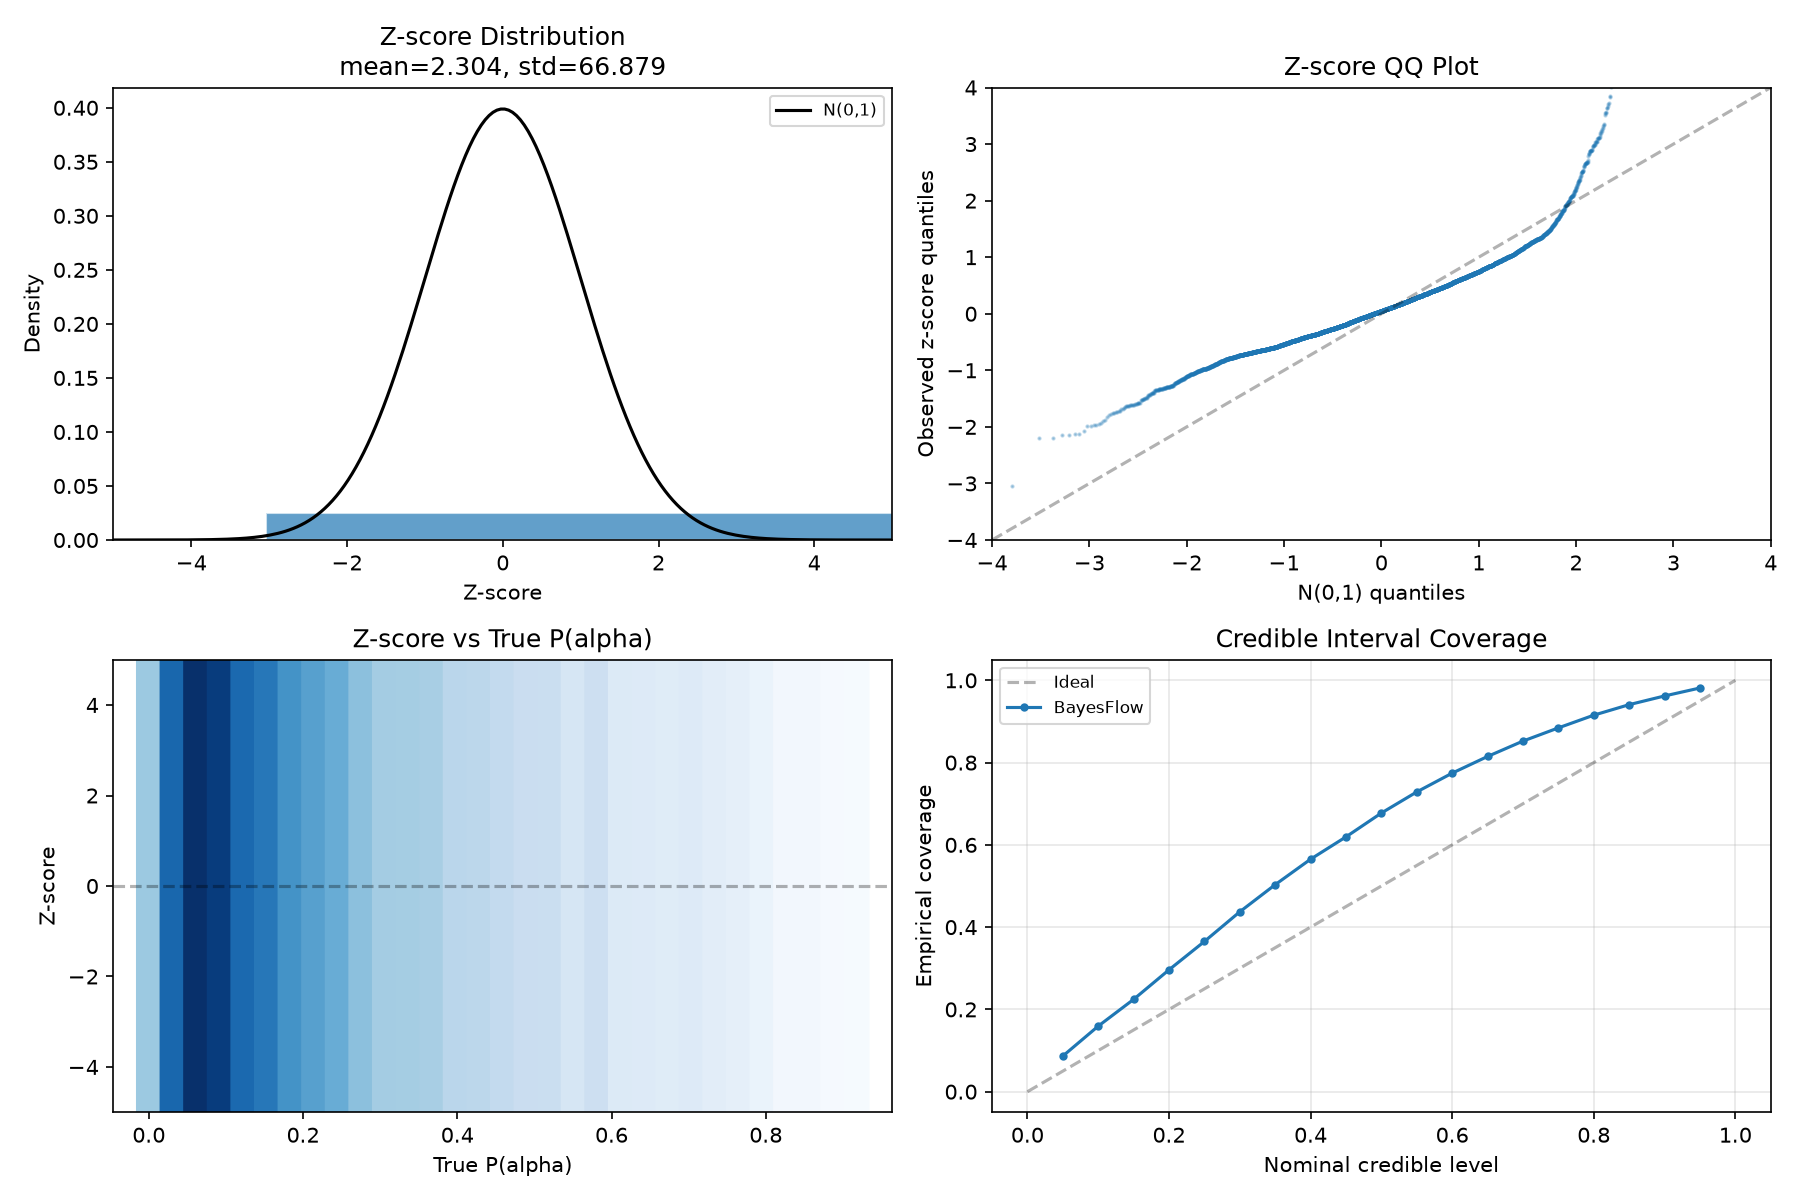
\includegraphics[width=\linewidth,height=0.62\textheight,keepaspectratio]{zscore_coverage.png}
\end{center}

\end{column}

% ----- RIGHT: Headline (30%) -----
\begin{column}{0.29\textwidth}

{\fontsize{9.0}{10.5}\selectfont
\textbf{\textcolor{red}{Undercoverage \& Bias}}
}

\vspace{0.12cm}

{\fontsize{7.5}{9.0}\selectfont
\textcolor{navy}{
Raw z-score std = \textbf{71.4}\\[3pt]
Trimmed (1.1\% outliers removed):\\[-0.3mm]
mean = \textbf{0.63},
std = \textbf{1.27}\\[6pt]
\textcolor{red}{87\% empirical vs.\ 90\% nominal}\\[1pt]
\textcolor{red}{93\% empirical vs.\ 95\% nominal}
}}

\vspace{0.25cm}

{\fontsize{7.5}{9.0}\selectfont
\textcolor{navy}{
Posteriors are \textbf{too narrow}\\[-0.3mm]
and \textbf{slightly biased}.\\[3pt]
$\to$ Localized overconfidence\\[-0.3mm]
at sequence boundaries.
}}

\end{column}

\end{columns}

\end{minipage}

\vfill
\hspace{0.95cm}
{\fontsize{5.5}{6.0}\selectfont\textcolor{gray}{SBI Project | 9/12}}
\vspace{0.26cm}

\end{frame}


% ================================================
% SLIDE 10 — Synthetic Evaluation: Posterior Contraction
% ================================================
\begin{frame}[plain]

\begin{tikzpicture}[remember picture,overlay]
  \fill[topgreen] (current page.north west) rectangle
    ([yshift=-0.13cm]current page.north east);
  \fill[navy] ([yshift=0.18cm]current page.south west) rectangle
    (current page.south east);
\end{tikzpicture}

\vspace{0.28cm}
\hspace{0.30cm}
\begin{minipage}{0.90\textwidth}

{\large\textbf{\textcolor{navy}{Synthetic Evaluation — Posterior Contraction}}}

\vspace{0.10cm}

\begin{columns}[T,totalwidth=\textwidth]

% ----- LEFT: Big Plot (70%) -----
\begin{column}{0.68\textwidth}

\begin{center}
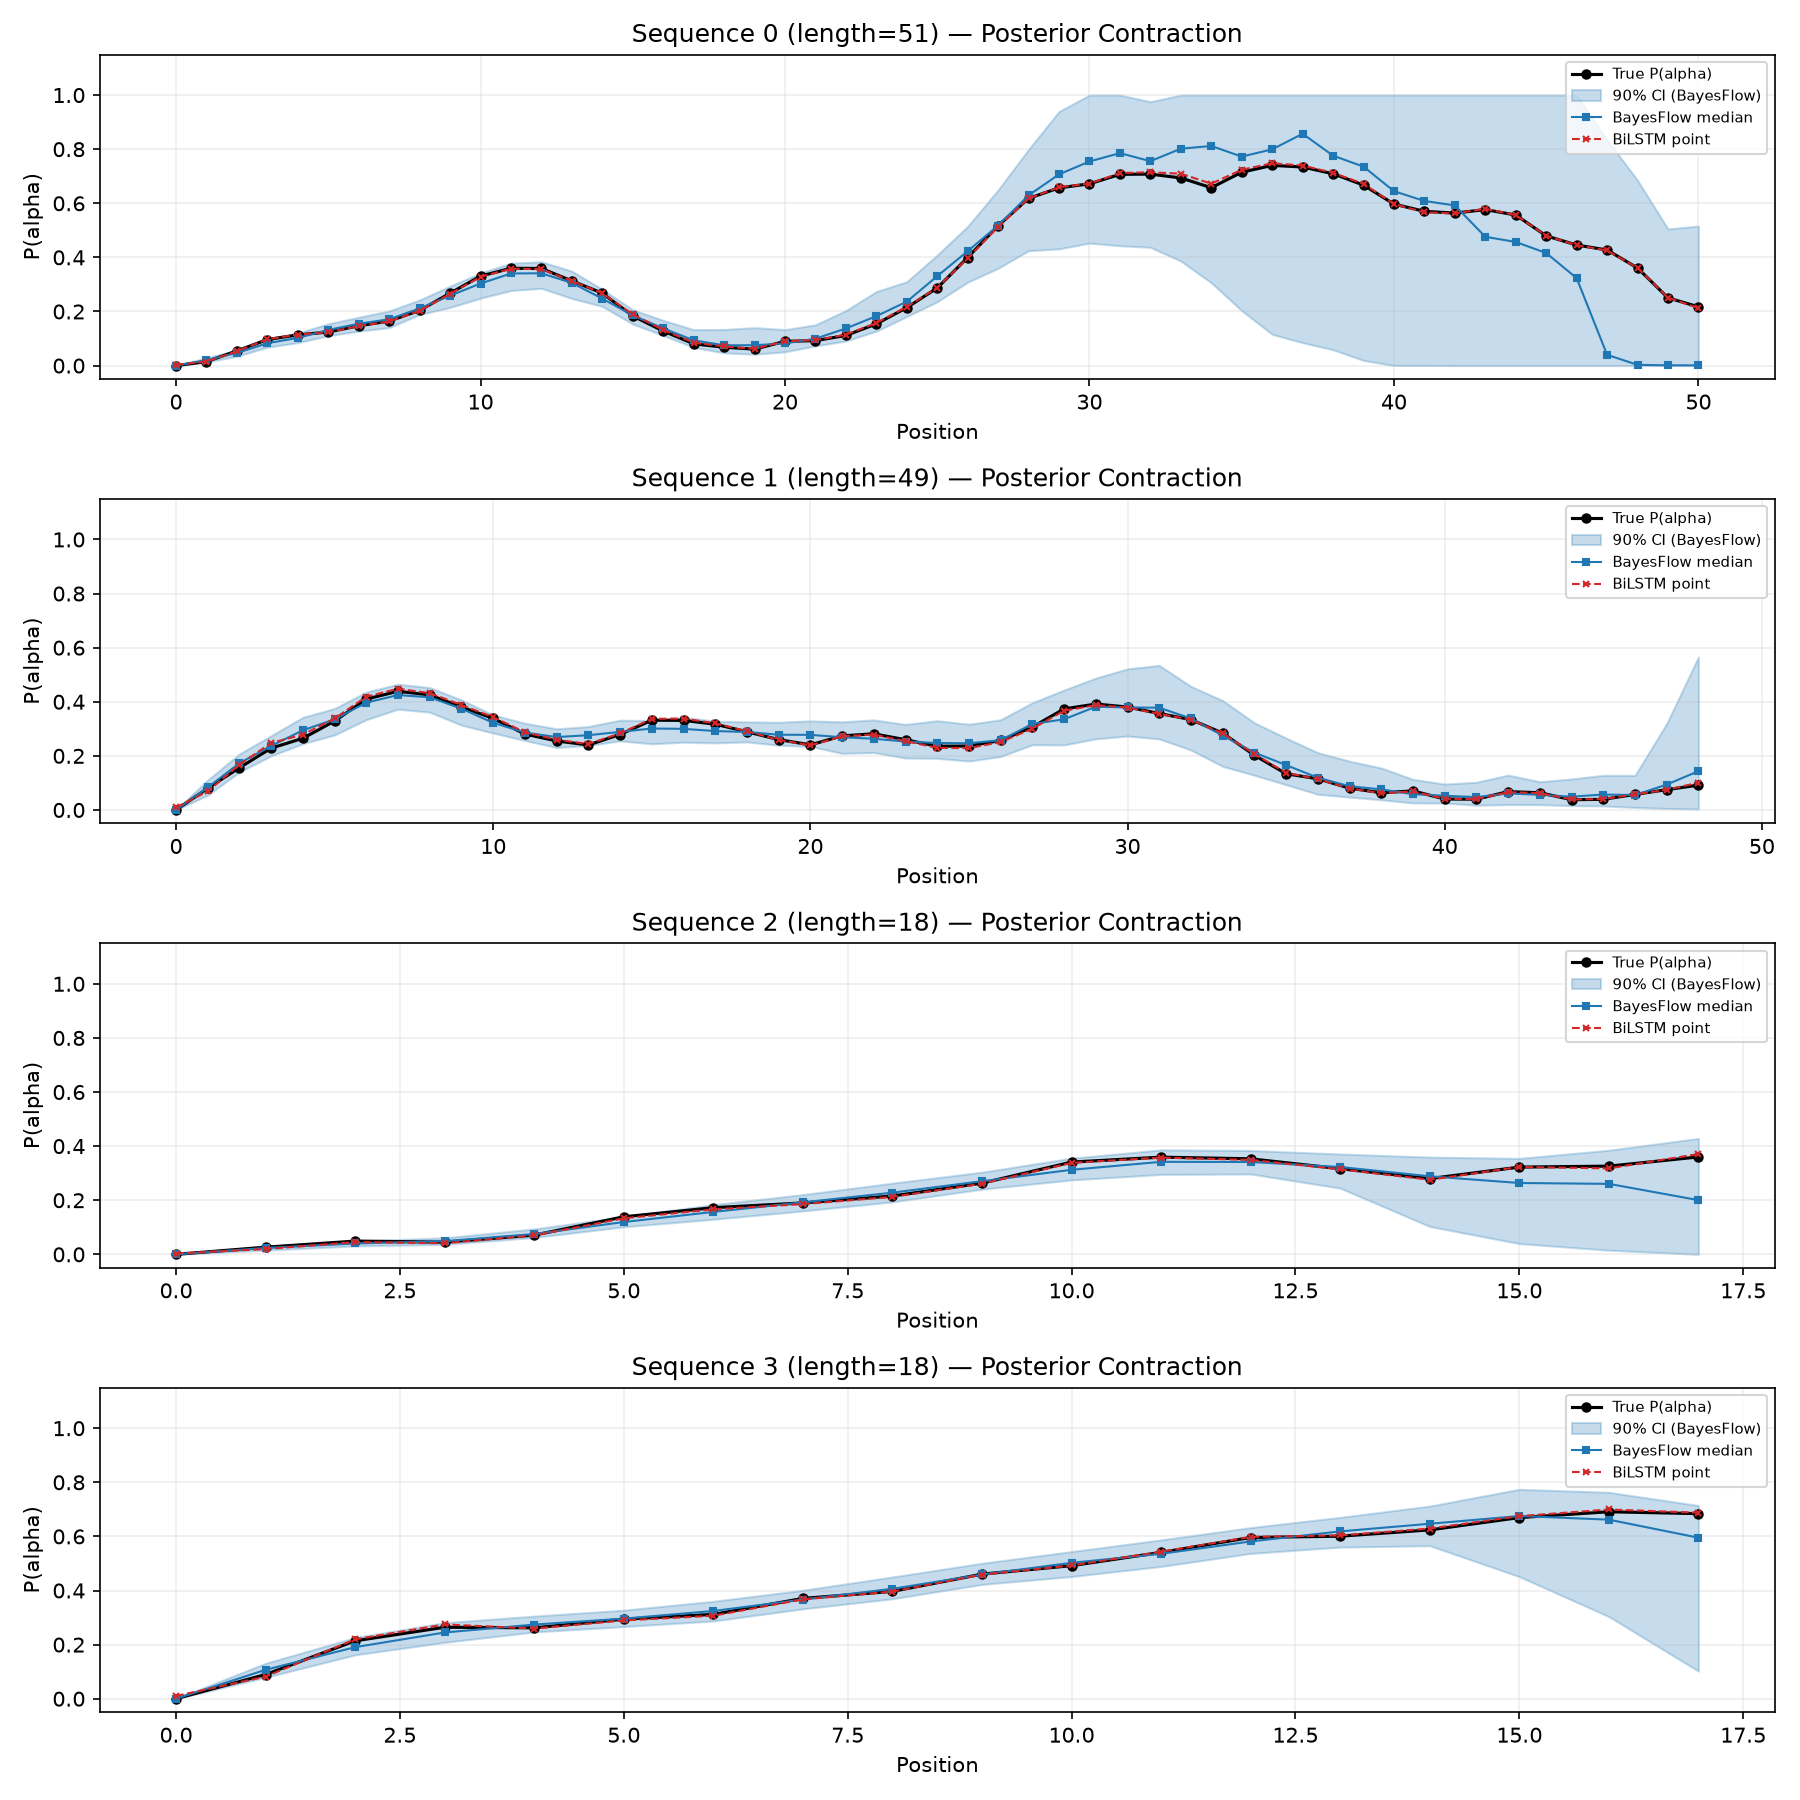
\includegraphics[width=\linewidth,height=0.62\textheight,keepaspectratio]{contraction.png}
\end{center}

\vspace{-0.10cm}

{\fontsize{5.5}{6.5}\selectfont
\textcolor{gray}{Black = true $P(\alpha)$. Blue band = 90\% CI. Red = BiLSTM point estimate.}
}

\end{column}

% ----- RIGHT: Headline (30%) -----
\begin{column}{0.29\textwidth}

{\fontsize{9.0}{10.5}\selectfont
\textbf{\textcolor{red}{BiLSTM Wins on Accuracy}}
}

\vspace{0.10cm}

{\fontsize{7.5}{9.0}\selectfont
\begin{tabular}{lcc}
\toprule
 & BayesFlow & BiLSTM \\
\midrule
MAE & 0.115 & \textbf{0.021} \\
Corr & 0.560 & \textbf{0.988} \\
\bottomrule
\end{tabular}
}

\vspace{0.18cm}

{\fontsize{7.5}{9.0}\selectfont
\textcolor{navy}{
FB target is \textbf{deterministic}\\[-0.3mm]
— direct network learns it\\[-0.3mm]
more efficiently than a\\[-0.3mm]
density estimator.
}}

\vspace{0.25cm}

{\fontsize{7.5}{9.0}\selectfont
\textcolor{darkgreen}{
\textbf{But:} BayesFlow gives\\[-0.3mm]
\textbf{uncertainty quantification}\\[-0.3mm]
— credible intervals,\\[-0.3mm]
SBC, z-scores, coverage.
}}

\end{column}

\end{columns}

\end{minipage}

\vfill
\hspace{0.95cm}
{\fontsize{5.5}{6.0}\selectfont\textcolor{gray}{SBI Project | 10/12}}
\vspace{0.26cm}

\end{frame}


% ================================================
% SLIDE 11 — Real-World Validation: Human Insulin 1A7F
% ================================================
\begin{frame}[plain]

\begin{tikzpicture}[remember picture,overlay]
  \fill[topgreen] (current page.north west) rectangle
    ([yshift=-0.13cm]current page.north east);
  \fill[navy] ([yshift=0.18cm]current page.south west) rectangle
    (current page.south east);
\end{tikzpicture}

\vspace{0.28cm}
\hspace{0.30cm}
\begin{minipage}{0.90\textwidth}

{\large\textbf{\textcolor{navy}{Real-World Validation — Human Insulin (1A7F)}}}

\vspace{0.10cm}

\begin{columns}[T,totalwidth=\textwidth]

% ----- LEFT: Big Plot (70%) -----
\begin{column}{0.68\textwidth}

\begin{center}
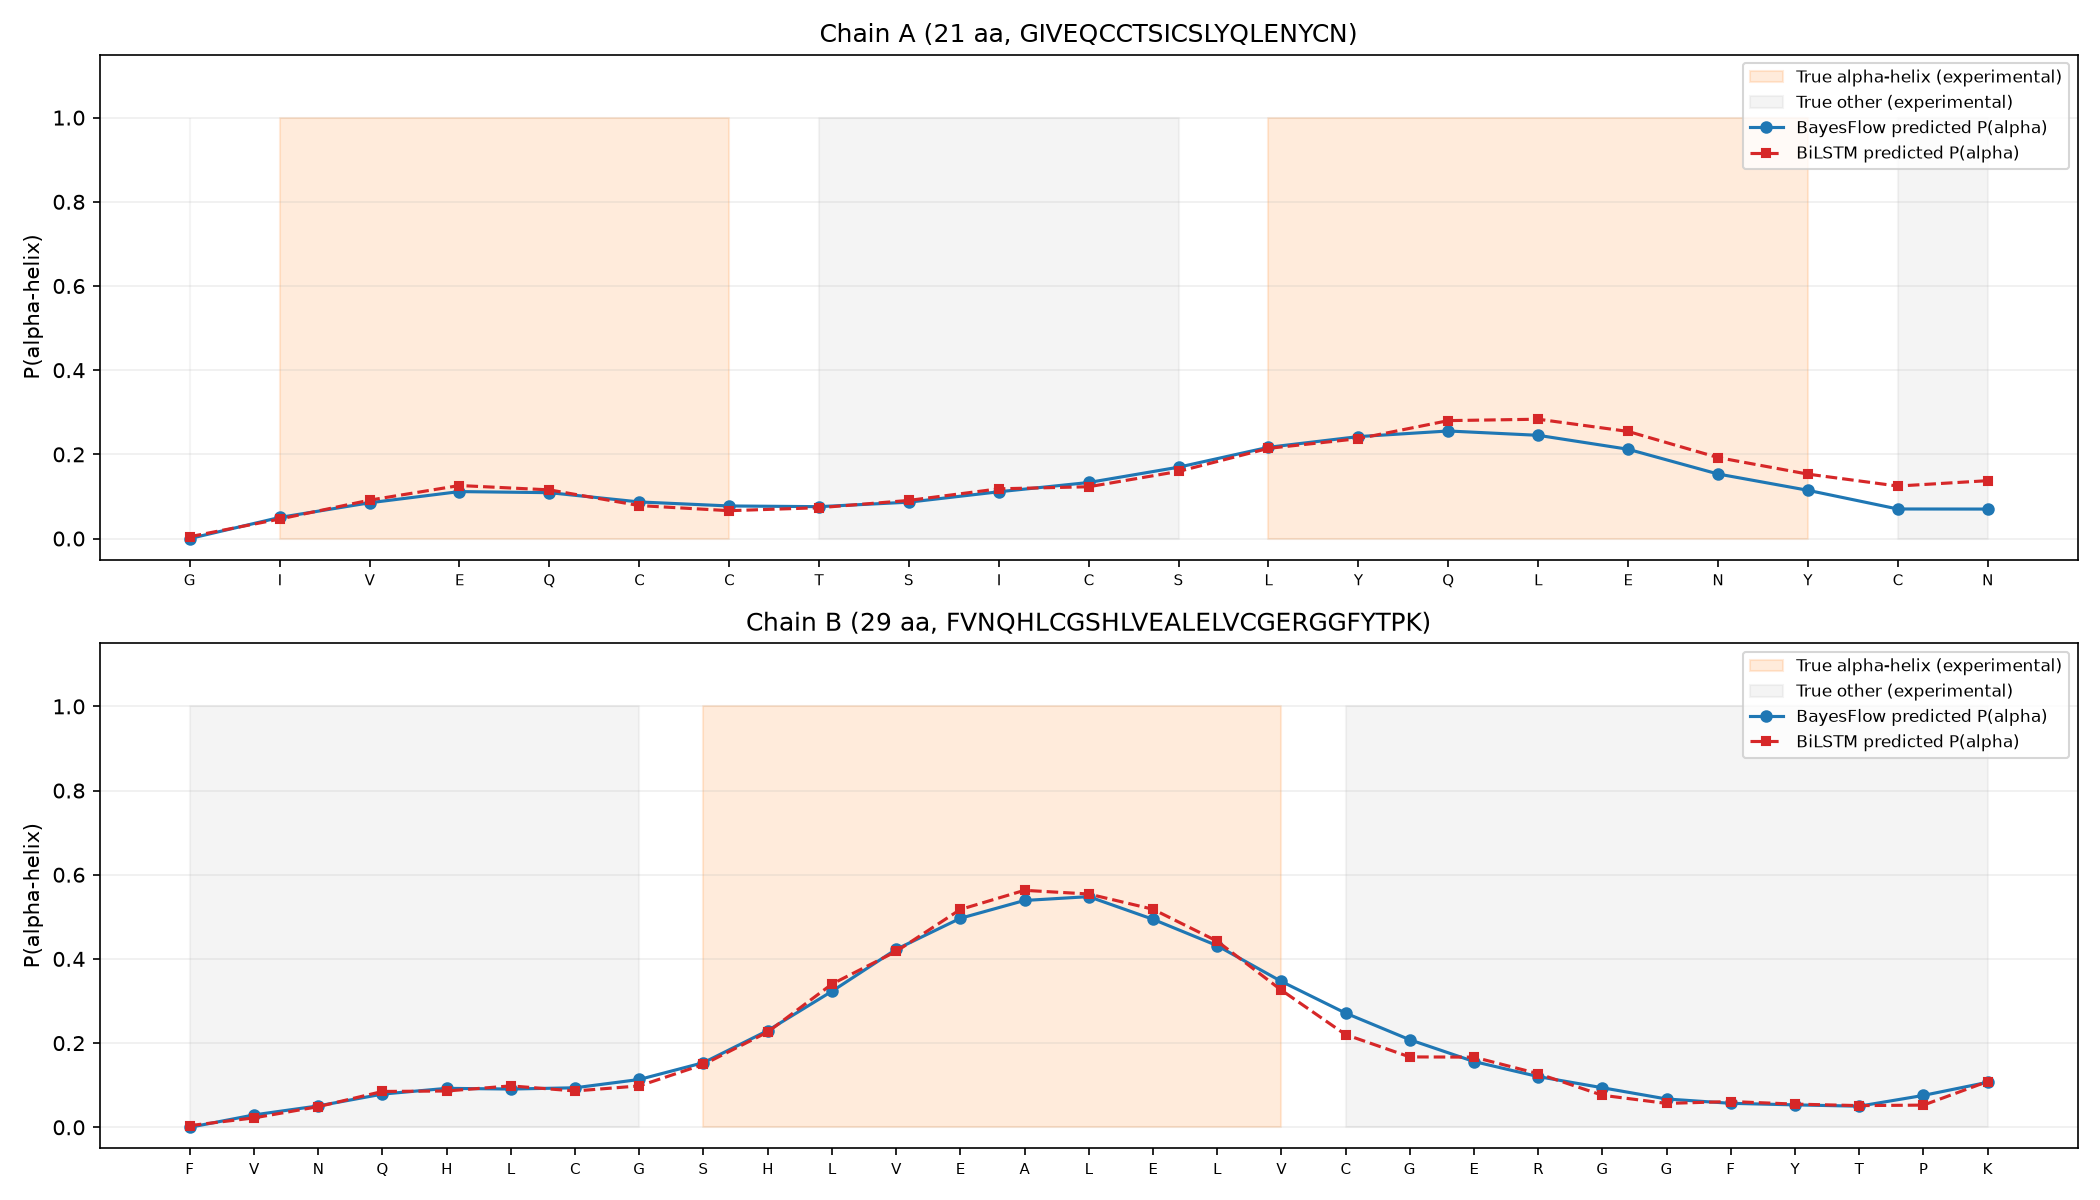
\includegraphics[width=\linewidth,height=0.62\textheight,keepaspectratio]{insulin_predictions.png}
\end{center}

\vspace{-0.10cm}

{\fontsize{5.5}{6.5}\selectfont
\textcolor{gray}{Orange = experimental $\alpha$-helix. Blue = BayesFlow. Red = BiLSTM.}
}

\end{column}

% ----- RIGHT: Headline (30%) -----
\begin{column}{0.29\textwidth}

{\fontsize{9.0}{10.5}\selectfont
\textbf{\textcolor{darkgreen}{Chain B}}
}

\vspace{0.06cm}

{\fontsize{7.5}{9.0}\selectfont
\textcolor{navy}{
BayesFlow\\[-0.3mm]
$r = \mathbf{0.86}$\\[2pt]
34.5\% true helix\\[1pt]
$\approx \pi = 33\%$
}}

\vspace{0.22cm}

{\fontsize{9.0}{10.5}\selectfont
\textbf{\textcolor{red}{Chain A}}
}

\vspace{0.06cm}

{\fontsize{7.5}{9.0}\selectfont
\textcolor{navy}{
BayesFlow\\[-0.3mm]
$r = \mathbf{0.17}$\\[2pt]
61.9\% true helix\\[1pt]
$\gg \pi = 33\%$
}}

\vspace{0.22cm}

{\fontsize{7.5}{9.0}\selectfont
\textcolor{darkgreen}{
\textbf{Key proof:} FB itself\\[-0.3mm]
fails on Chain A\\[-0.3mm]
($r \approx 0.40$).\\[3pt]
$\to$ \textbf{Model limitation,}\\[-0.3mm]
\textbf{not network failure.}
}}

\end{column}

\end{columns}

\end{minipage}

\vfill
\hspace{0.95cm}
{\fontsize{5.5}{6.0}\selectfont\textcolor{gray}{SBI Project | 11/12}}
\vspace{0.26cm}

\end{frame}


% ================================================
% SLIDE 12 — Limitations, Fixes & TL;DR
% ================================================
\begin{frame}[plain]

\begin{tikzpicture}[remember picture,overlay]
  \fill[topgreen] (current page.north west) rectangle
    ([yshift=-0.13cm]current page.north east);
  \fill[navy] ([yshift=0.18cm]current page.south west) rectangle
    (current page.south east);
\end{tikzpicture}

\vspace{0.28cm}
\hspace{0.30cm}
\begin{minipage}{0.90\textwidth}

{\large\textbf{\textcolor{navy}{Limitations, Fixes \& Take-Home Messages}}}

\vspace{0.15cm}

\begin{columns}[T,totalwidth=\textwidth]

% ----- LEFT: Content -----
\begin{column}{0.60\textwidth}

{\fontsize{8.0}{9.5}\selectfont
\textbf{\textcolor{red}{Limitation \& Fix: The HMM}}
}

\vspace{0.04cm}

{\fontsize{6.8}{8.0}\selectfont
\textcolor{navy}{
Expand to \textbf{3 states} ($\alpha$, $\beta$, coil).\\[2pt]
Treat transition probabilities as \textbf{inferable}\\[-0.5mm]
parameters $\boldsymbol{\theta}$ under Beta priors.\\[2pt]
$\to$ BayesFlow would then recover a genuine posterior over $\boldsymbol{\theta}$.
}}

\vspace{0.10cm}

{\fontsize{8.0}{9.5}\selectfont
\textbf{\textcolor{red}{Fix: The CouplingFlow}}
}

\vspace{0.04cm}

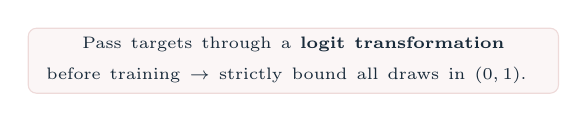
\begin{tikzpicture}
\node[fill=red!5, draw=red!20, rounded corners=3pt,
      line width=0.4pt, text width=6.5cm, minimum height=0.65cm, align=center]{
{\fontsize{6.5}{7.5}\selectfont
\textcolor{navy}{
Pass targets through a \textbf{logit transformation}\\[-0.3mm]
before training $\to$ strictly bound all draws in $(0,1)$.
}}
};
\end{tikzpicture}

\vspace{0.10cm}

{\fontsize{8.0}{9.5}\selectfont
\textbf{\textcolor{darkgreen}{Take-Home Messages (TL;DR)}}
}

\vspace{0.06cm}

{\fontsize{6.8}{8.0}\selectfont
\textcolor{navy}{
\textbf{1.} BiLSTM summary nets capture sequential\\[-0.3mm]
\ \ dependencies where permutation-invariant nets fail.\\[4pt]
\textbf{2.} BayesFlow successfully amortizes posterior\\[-0.3mm]
\ \ estimation, enabling robust uncertainty quantification.\\[4pt]
\textbf{3.} Real-world validation demonstrates the necessity\\[-0.3mm]
\ \ of prior typicality checking — identify prior-data conflicts.
}}

\end{column}

% ----- RIGHT: Group Members -----
\begin{column}{0.37\textwidth}

{\fontsize{8.0}{9.5}\selectfont
\textbf{\textcolor{darkgreen}{Group Members}}
}

\vspace{0.10cm}

{\fontsize{6.5}{7.5}\selectfont
\textcolor{navy}{
\textbf{Armin Maddah Asl}\\[-0.5mm]
\footnotesize\textcolor{gray}{armin.maddah@tu-dortmund.de}\\[6pt]
\textbf{Samaneh Naghdbishi}\\[-0.5mm]
\footnotesize\textcolor{gray}{samaneh.naghdbishi@tu-dortmund.de}\\[6pt]
\textbf{Kiana Ebrahimi Farbod}\\[-0.5mm]
\footnotesize\textcolor{gray}{kiana.ebrahimi@tu-dortmund.de}\\[6pt]
\textbf{Geri Lila}\\[-0.5mm]
\footnotesize\textcolor{gray}{geri.lila@tu-dortmund.de}
}}

\vspace{0.18cm}

% Repo link
{\fontsize{6.5}{7.5}\selectfont
\textcolor{gray}{\textbf{Code:}}\\[2pt]
\footnotesize\textcolor{blue}{\url{github.com/armin2080/protein-secondary-structure-npe}}
}

\end{column}

\end{columns}

\end{minipage}

\vfill
\hspace{0.95cm}
{\fontsize{5.5}{6.0}\selectfont\textcolor{gray}{SBI Project | 12/12}}
\vspace{0.26cm}

\end{frame}


\end{document}
